% -*- TeX-master: "oving03"; -*-
\oppgaver{4}

\begin{oppgave}
Finn ut om følgende påstander er sanne eller ikke.
\begin{punkt}
Hvis tre vektorer $\V{u}$, $\V{v}$ og~$\V{w}$ er lineært
avhengige, så finnes det to tall $a$ og~$b$ slik at: 
\[
\V{u} = a \cdot \V{v} + b \cdot \V{w}
\]
\end{punkt}
\end{oppgave}


\begin{oppgave}
De to bildene viser vektorer i $\mathbb{R} ^2$. 
	
\begin{punkt}
Er vektorene $\V{v}_1$ og~$\V{v}_2$ lineært uavhengige? Utspenner de $\mathbb{R} ^2$? Begrunn svarene dine.
\begin{center}
	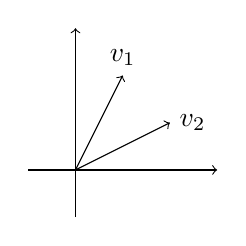
\begin{tikzpicture}[scale=0.6]
	\draw[->,above] (0,0) node{} -- (1,2) node{$\V{v}_1$};
	\draw[->, right] (0,0) node{} -- (2,1) node{$\V{v}_2$};
	\draw[->] (-1,0) {} -- (3,0) {};
	\draw[->] (0,-1) {} -- (0,3) {};
	\end{tikzpicture}
\end{center}
\end{punkt}



\begin{punkt}
Er vektorene $\V{v}_1$, $\V{v}_2$ og~$\V{v}_3$ lineært uavhengige? Utspenner de $\mathbb{R} ^2$? Begrunn svarene dine.
\begin{center}
	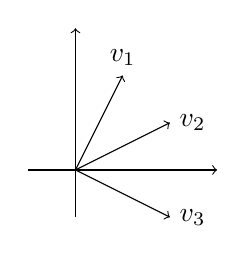
\begin{tikzpicture}[scale=0.6]
	\draw[->,above] (0,0) node{} -- (1,2) node{$\V{v}_1$};
	\draw[->, right] (0,0) node{} -- (2,1) node{$\V{v}_2$};
	\draw[->, right] (0,0) node{} -- (2,-1) node{$\V{v}_3$};
	\draw[->] (-1,0) {} -- (3,0) {};
	\draw[->] (0,-1) {} -- (0,3) {};
	\end{tikzpicture}
\end{center}
\end{punkt}
\end{oppgave}

\begin{oppgave}
\begin{punkt}
Betrakt vektorene
\[ 
\begin{bmatrix} \;1\; \\ \;2\; \end{bmatrix}, 
\begin{bmatrix} \;2\; \\ \;3\; \end{bmatrix}, \dots, 
\begin{bmatrix} \;99\; \\ \;100\; \end{bmatrix}
\]
i $\mathbb{R}^2$. Vis at de utspenner $\mathbb{R}^2$. Er de lineært uavhengig? Begrunn svaret ditt.
\end{punkt}

\begin{punkt}
Betrakt vektorene
\[ 
\begin{bmatrix} 
\;1\; \\ 
\;\vdots\; \\ 
\;99\; 
\end{bmatrix}
\text{ og }
\begin{bmatrix} 
\;2\; \\ 
\;\vdots\; \\ 
\;100\; 
\end{bmatrix}
\]
i $\mathbb{R}^{99}$. Er de lineært uavhengige? Begrunn svaret ditt.

\end{punkt}
\end{oppgave}